% Standalone A1 landscape poster. All diagrams are vector graphics in this file.
% Export: pdflatex -interaction=nonstopmode -halt-on-error -jobname=resumelens-poster-latex -output-directory=output/pdf docs/resumelens-poster.tex
\documentclass{article}
\usepackage[T1]{fontenc}
\usepackage[utf8]{inputenc}
\usepackage{lmodern}
\usepackage[paperwidth=841mm,paperheight=594mm,margin=18mm]{geometry}
\usepackage{amsmath,amssymb,xcolor,tikz,tabularx,array}
\usetikzlibrary{arrows.meta,positioning,automata}
\newcommand{\href}[2]{#2}
\definecolor{navy}{HTML}{17324D}
\definecolor{blue}{HTML}{0A66C2}
\definecolor{pale}{HTML}{EEF4FA}
\definecolor{ink}{HTML}{243746}
\definecolor{green}{HTML}{16734B}
\pagestyle{empty}
\setlength{\parindent}{0pt}
\setlength{\parskip}{5mm}
\setlength{\fboxsep}{7mm}
\DeclareMathSizes{21}{21}{16}{12}
\newcommand{\heading}[2]{\par\vspace{4mm}{\sffamily\bfseries\fontsize{29}{34}\selectfont\color{blue}#1\quad #2}\par\vspace{2mm}{\color{blue}\hrule height 1.5pt}\vspace{5mm}}
\newcommand{\subhead}[1]{{\sffamily\bfseries\color{navy}#1}\par\vspace{1mm}}
\newcommand{\token}[1]{\texttt{#1}}
\newcommand{\note}[1]{\par\colorbox{pale}{\parbox{\dimexpr\linewidth-2\fboxsep\relax}{#1}}\par}
\ifdefined\pdfinfo
\pdfinfo{/Title (ResumeLens: Formal Language-Based Resume Screening) /Author (Victor Team)}
\fi
\begin{document}
\color{ink}\fontsize{21}{27}\selectfont
\noindent\colorbox{navy}{\parbox{\dimexpr\textwidth-2\fboxsep\relax}{
  \color{white}{\sffamily\bfseries\fontsize{67}{74}\selectfont ResumeLens}\hfill
  {\sffamily\fontsize{23}{28}\selectfont V\'ictor Team}\par
  \vspace{2mm}{\sffamily\fontsize{37}{43}\selectfont Formal Language-Based Resume Screening}\par
  \vspace{4mm}{\fontsize{23}{29}\selectfont Explicit evidence \enspace$\longrightarrow$\enspace canonical skills \enspace$\longrightarrow$\enspace explainable patterns \enspace$\longrightarrow$\enspace validated profiles}\par
  \vspace{2mm}{\sffamily\fontsize{19}{24}\selectfont Discrete Structures III \enspace$\vert$\enspace Integrative Task \enspace$\vert$\enspace October 2026}
}}
\vspace{9mm}

\noindent\begin{minipage}[t]{0.315\textwidth}
\heading{01}{Problem and objective}
R\'esum\'es express equivalent skills using different names and place them in different orders. ResumeLens tests whether \textbf{explicitly reported qualifications} satisfy a defined professional pattern.

\note{\textbf{Research question}\par
How can regular expressions, finite-state transducers, finite automata and a structured language form one traceable r\'esum\'e-processing pipeline?}

\subhead{Four profiles, one solution}
Full Stack Developer and Machine Learning Engineer are the reference profiles. Cloud \& DevOps Engineer and Data Scientist are the team's additional profiles.

\heading{02}{Shared architecture}
\begin{center}
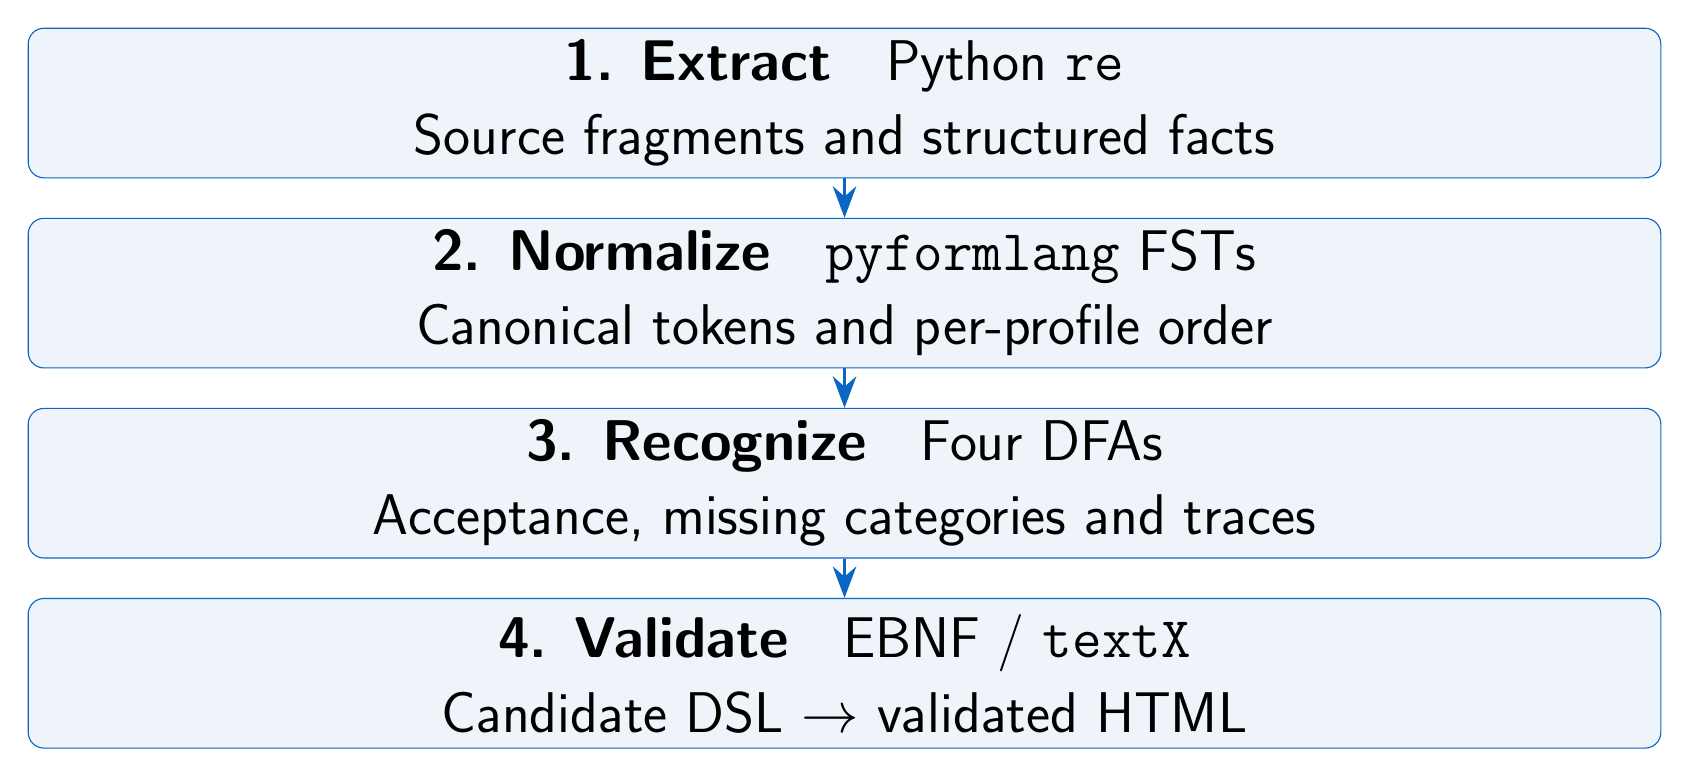
\begin{tikzpicture}[node distance=5mm,box/.style={draw=blue,fill=pale,rounded corners=2mm,text width=205mm,minimum height=19mm,align=center,font=\sffamily\fontsize{22}{27}\selectfont},arr/.style={-{Stealth[length=4mm]},thick,blue}]
\node[box] (a) {\textbf{1. Extract}\quad Python \token{re}\\Source fragments and structured facts};
\node[box,below=of a] (b) {\textbf{2. Normalize}\quad \token{pyformlang} FSTs\\Canonical tokens and per-profile order};
\node[box,below=of b] (c) {\textbf{3. Recognize}\quad Four DFAs\\Acceptance, missing categories and traces};
\node[box,below=of c] (d) {\textbf{4. Validate}\quad EBNF / \token{textX}\\Candidate DSL $\rightarrow$ validated HTML};
\draw[arr] (a)--(b);\draw[arr] (b)--(c);\draw[arr] (c)--(d);
\end{tikzpicture}
\end{center}
\token{src/pipeline.py} orchestrates the four stages. React and Streamlit present the same Python results; the browser does not reproduce the classification rules.

\heading{03}{Extraction with regex}
The extractor preserves source mentions, finds section boundaries and resolves overlapping matches. Contact spans are protected from accidental skill extraction.

\textbf{Context matters:} ambiguous names are restricted to skill sections. A longer mention such as \token{GitHub Actions} takes precedence over the overlapping \token{GitHub} match.

Results remain in a structured data model and can be saved as JSON. Extraction records evidence; it does not decide profile acceptance.
\end{minipage}\hfill
\begin{minipage}[t]{0.315\textwidth}
\heading{04}{Normalization with FSTs}
The cascade \textbf{CLEAN $\rightarrow$ ALIAS}, plus an EXPERIENCE transducer, maps textual variants to canonical symbols. FILTER passes prepare a separate order for each profile.
\[
 T=(Q,\Sigma,\Gamma,\delta,\omega,q_0,F)
\]
Here $\Sigma$ and $\Gamma$ are input and output alphabets; $\delta$ specifies transitions and $\omega$ their outputs. The transducers execute in \token{pyformlang}.

\note{\token{JS} $\mapsto$ \token{JAVASCRIPT}\qquad
\token{React.js} $\mapsto$ \token{REACT}\par
\token{NodeJS} $\mapsto$ \token{NODE\_JS}\qquad
\token{Postgres} $\mapsto$ \token{POSTGRESQL}}

Exact years remain metadata; positive experience is abstracted as the finite symbol \token{EXPERIENCE\_PRESENT}. Unknown skills remain visible.

\heading{05}{Recognition with four DFAs}
Each profile has a deterministic, total automaton with an explicit trap state:
\[
 M_i=(Q_i,\Sigma_i,\delta_i,q_0,F_i),
 \qquad \delta_i:Q_i\times\Sigma_i\to Q_i.
\]
Acceptance means membership in the profile language:
\[
 w_i\in L(M_i)\iff\delta_i^*(q_0,w_i)\in F_i.
\]
The prepared sequence $w_i$ contains relevant skills in that profile's category order. A candidate may satisfy several profiles.

\subhead{Machine Learning: accepted trace}
\begin{center}
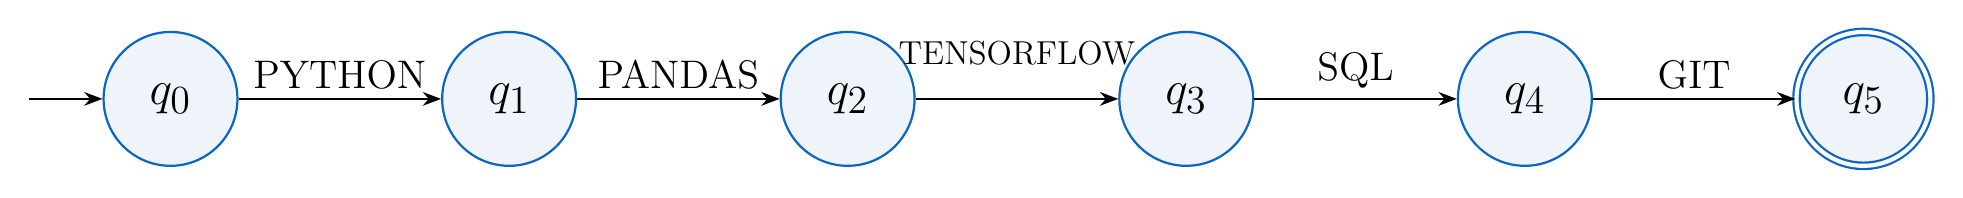
\begin{tikzpicture}[x=1mm,y=1mm,>=Stealth,thick,every node/.style={font=\fontsize{19}{23}\selectfont},state/.style={circle,draw=blue,fill=pale,minimum size=17mm,inner sep=0pt}]
\node[state] (q0) at (0,0) {$q_0$};
\node[state] (q1) at (43,0) {$q_1$};
\node[state] (q2) at (86,0) {$q_2$};
\node[state] (q3) at (129,0) {$q_3$};
\node[state] (q4) at (172,0) {$q_4$};
\node[state,double,double distance=1.5pt] (q5) at (215,0) {$q_5$};
\draw[->] (-18,0)--(q0);
\draw[->] (q0)--node[above,font=\fontsize{15}{19}\selectfont]{PYTHON}(q1);
\draw[->] (q1)--node[above,font=\fontsize{15}{19}\selectfont]{PANDAS}(q2);
\draw[->] (q2)--node[above=3mm,font=\fontsize{12}{16}\selectfont]{TENSORFLOW}(q3);
\draw[->] (q3)--node[above,font=\fontsize{15}{19}\selectfont]{SQL}(q4);
\draw[->] (q4)--node[above,font=\fontsize{15}{19}\selectfont]{GIT}(q5);
\end{tikzpicture}
\end{center}
{\fontsize{18}{23}\selectfont One accepted path, with shortened state labels. Category loops and trap transitions are omitted here; complete models are in the repository.}

\subhead{Pattern decisions}
Full Stack requires frontend, backend, database and version-control evidence, with defined alternatives and optional categories. The other three profiles require every category in their respective patterns.

Strict token mode preserves order: an out-of-order or foreign symbol reaches the trap state. R\'esum\'e mode prepares each profile's input first.
\end{minipage}\hfill
\begin{minipage}[t]{0.315\textwidth}
\heading{06}{A validated candidate language}
The DSL represents personal data, contacts, experience, education, skills and accepted profiles. Repeated records are supported.

\note{{\ttfamily\fontsize{19}{25}\selectfont
candidate \{\par
\quad personal \{ name "Wednesday Addams"; \}\par
\quad contact \{ \}\par
\quad experience \{ total\_years 3; \}\par
\quad education \{ \}\par
\quad skills \{ skill JAVASCRIPT; \ldots\ \}\par
\quad classification \{ accepted full\_stack; \}\par
\}}\par
{\fontsize{17}{22}\selectfont Abbreviated illustration; the ellipsis is not valid DSL syntax.}}

\token{textX} parses the document and domain checks enforce valid contacts, vocabulary and uniqueness. \textbf{HTML is generated only after validation}; values are escaped. Its runtime parser uses PEG semantics, while the language structure is documented in EBNF.

\heading{07}{Results and evidence}
\begin{center}
{\sffamily\bfseries\fontsize{65}{70}\selectfont\color{green}883}\par
{\sffamily\fontsize{24}{29}\selectfont automated tests passing}
\end{center}
\textbf{Verified 11 October 2026:} extraction boundaries, alias transduction, canonical order, DFA acceptance and rejection, DSL errors, HTML generation and API integration. The React production build also compiles.

\subhead{End-to-end example}
\token{JS, React.js, NodeJS, Postgres, Git}\par
$\Downarrow$\quad extraction and FST normalization\par
\token{JAVASCRIPT, REACT, NODE\_JS,}\par
\token{POSTGRESQL, GIT}\par
$\Downarrow$\quad Full Stack DFA accepts\par
Validated candidate DSL $\longrightarrow$ HTML profile.

\heading{08}{Limits and next steps}
Rule coverage limits extraction; negation and skill proficiency are not modeled. Employers, institutions and periods are not reliably reconstructed. Grammar validity does not establish factual truth, and acceptance does not rank candidates.

\textbf{Next evaluation:} an annotated r\'esum\'e corpus to measure extraction precision and recall. Passing tests are evidence of programmed behavior, not recruitment accuracy.

\heading{}{Selected references}
{\fontsize{17}{22}\selectfont
[1] J. Romero. \emph{Pyformlang: An Educational Library for Formal Language Manipulation}. SIGCSE, 2021. \href{https://doi.org/10.1145/3408877.3432464}{doi:10.1145/3408877.3432464}.\par
[2] I. Dejanovi\'c et al. \emph{TextX: A Python tool for Domain-Specific Languages implementation}. Knowledge-Based Systems 115, 2017. \href{https://doi.org/10.1016/j.knosys.2016.10.023}{doi:10.1016/j.knosys.2016.10.023}.\par
[3] Python Software Foundation, \emph{re documentation}; textX contributors, \emph{Grammar and Meta-model documentation}. Full review: \token{docs/literature\_review.md}.
}
\end{minipage}
\vfill
{\color{blue}\hrule height 1.5pt}\vspace{4mm}
{\sffamily\fontsize{19}{24}\selectfont\textbf{Reproducible implementation and complete formal models}\hfill
\href{https://github.com/JuanJoe-18/DiscreteIII-Integrative-Task-VictorTeam}{github.com/JuanJoe-18/DiscreteIII-Integrative-Task-VictorTeam}}
\end{document}
